\documentclass[10pt]{article}
\usepackage[margin=1in]{geometry}
\usepackage{booktabs}
\usepackage{array}
\usepackage{longtable}
\usepackage{graphicx}
\usepackage{xurl}
\usepackage{fvextra}
\usepackage{fontspec}
\setmonofont{DejaVu Sans Mono}
\usepackage[hidelinks]{hyperref}
\setlength{\parskip}{6pt}
\setlength{\parindent}{0pt}
\begin{document}

\begin{center}
{\Large \textbf{Supplementary Information}}\\[4pt]
{\large DB-Curator: On-demand scientific database curation via deep-research multi-agent literature mining and verification}
\end{center}

\section*{Supplementary Figure 1. Detailed DB-Curator workflow}

\begin{center}
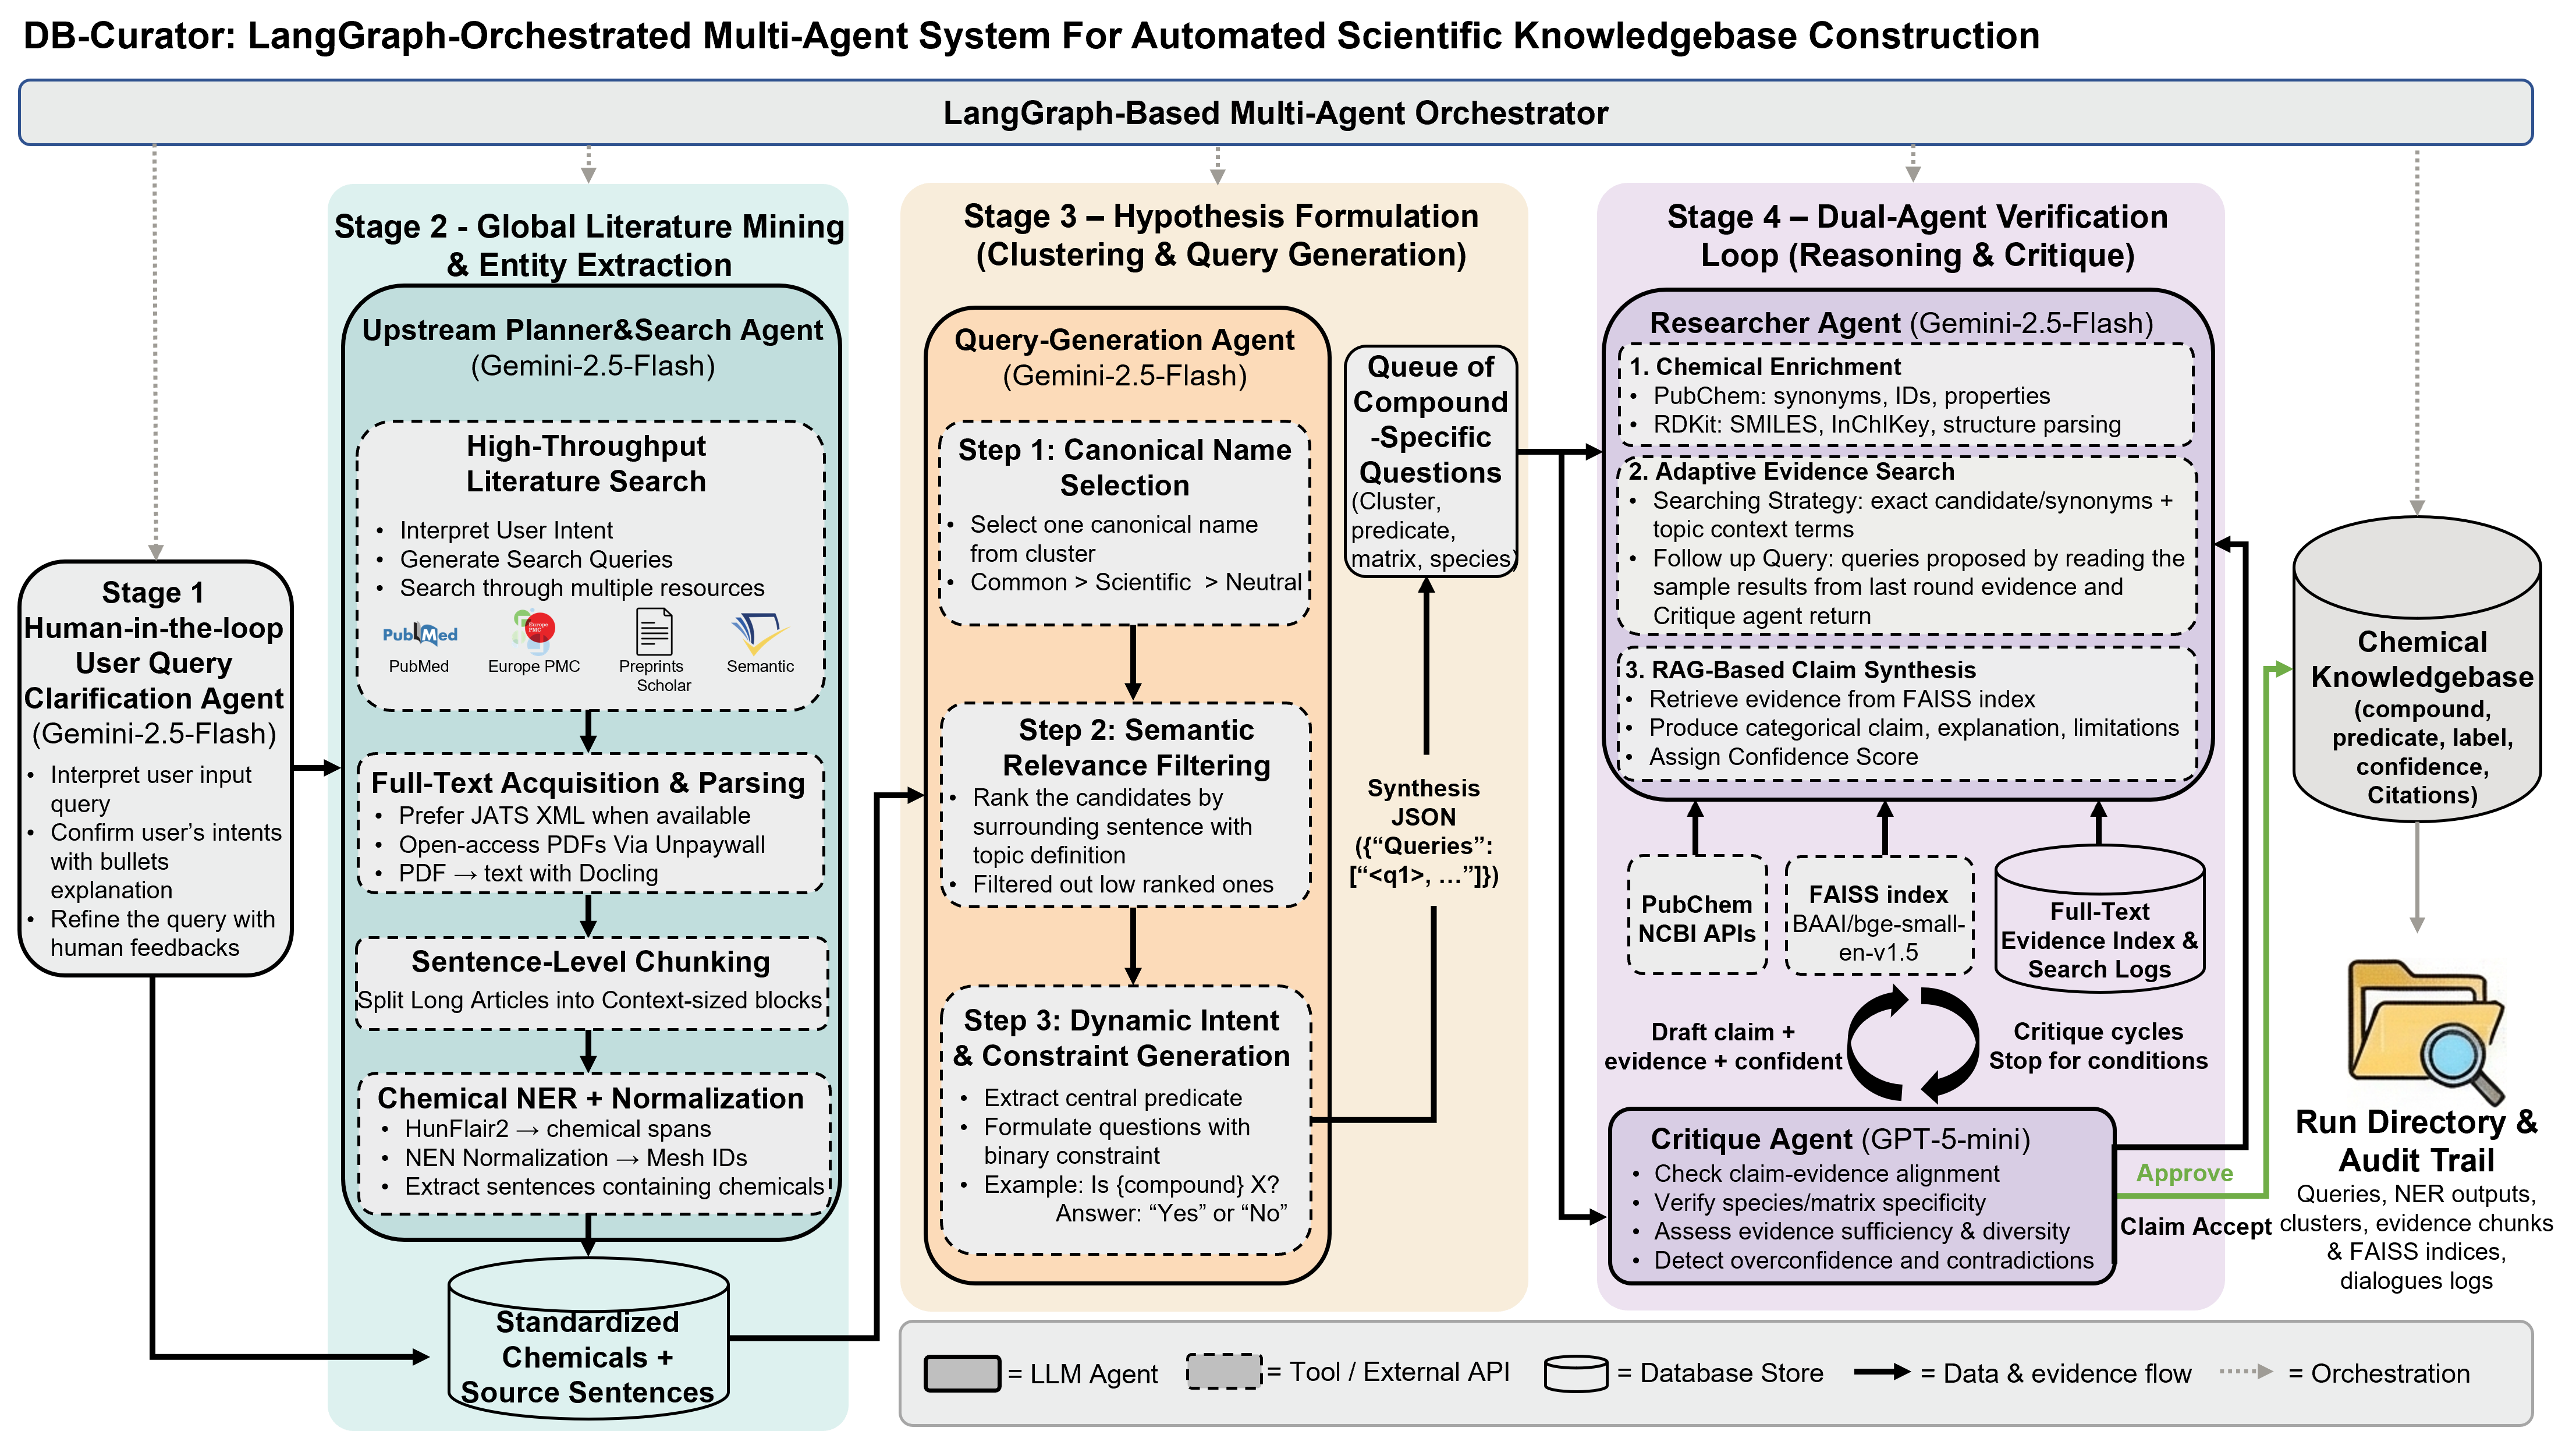
\includegraphics[width=\linewidth]{vertopal_348d7636602e415aacb4c9f4c07d6a38/media/SI_workflow.png}
\end{center}

Supplementary Figure 1 \textbar{} Expanded workflow for DB-Curator, showing
how user-defined scope, dynamic literature construction, chemical candidate
discovery, candidate filtering, predicate-state verification, critique-guided
follow-up, and provenance export are connected in the full curation system.

\section*{Supplementary Note 1. Topic definitions used for evaluation}

DB-Curator was evaluated with explicit user-defined topic definitions. These definitions were used to build the verification rubrics and to guide manual inspection of non-overlap outputs.

\begin{longtable}{@{}>{\raggedright\arraybackslash}p{0.14\linewidth}>{\raggedright\arraybackslash}p{0.80\linewidth}@{}}
\toprule
Topic & User-defined topic scope \\
\midrule
DBPs & A disinfection by-product is a specific chemical compound formed when disinfectants or oxidants react with natural or anthropogenic precursors in real or simulated water matrices, with direct evidence attributing formation to the treatment process. \\
Blood exposome & A human blood exposome chemical is a specific chemical entity reported in human blood or systemic circulation that is introduced by, structurally modified by, or significantly changes in amount in response to the external environment, and is supported by evidence from primary literature, biomonitoring surveys, or public metabolomics datasets associated with human blood specimens. \\
Drug compounds & A drug compound is a core active drug substance or drug entity represented in a drug database, including small-molecule and biologic drugs, that elicits or is intended to elicit pharmacologically relevant effects, while excluding specific finished dosage forms, secondary brand names, and other non-active product-level entries. \\
Human endogenous metabolites & A human endogenous metabolite is a specific small-molecule metabolite produced within the human body and functioning in biochemical and physiological processes, while excluding exogenous chemicals and microbiota-only metabolites unless they are also produced by host metabolism. \\
Microbial natural products & A microbial natural product is a specific chemical metabolite produced by microorganisms, such as bacteria, fungi, or cyanobacteria, curated from peer-reviewed primary scientific literature and supported by sufficient analytical evidence for unambiguous structural assignment, while excluding primary metabolites and non-secondary-metabolite biomolecules. \\
\bottomrule
\end{longtable}

\section*{Supplementary Note 2. Benchmark resources}

The five benchmark resources were used for identity overlap analysis and benchmark-scale verification. DBP used the full curated benchmark available for this study. For the other four resources, 300 candidate rows were sampled with fixed seeds from the source database to provide comparable benchmark-scale evaluation sets.

\begin{longtable}{p{0.18\linewidth}p{0.34\linewidth}p{0.38\linewidth}}
\toprule
Topic & Benchmark source & Role in evaluation \\
\midrule
DBP & Systematic DBP curation resource with 687 compounds & Full benchmark-scale verification and fixed-cohort overlap analysis. \\
Blood exposome & Blood Exposome Database, July 2023 chemical list & Random 300-row benchmark-scale verification set and fixed-cohort overlap analysis. \\
Drug compounds & DrugBank structure and vocabulary exports & Random 300-row benchmark-scale verification set and fixed-cohort overlap analysis. \\
Human endogenous metabolites & HMDB metabolite export & Random 300-row benchmark-scale verification set and fixed-cohort overlap analysis. \\
Microbial natural products & Natural Products Atlas export & Random 300-row benchmark-scale verification set and fixed-cohort overlap analysis. \\
\bottomrule
\end{longtable}

\section*{Supplementary Note 3. Manual inspection and release rule}

For fixed-cohort release evaluation, benchmark-overlap rows were automatically accepted because their normalized compound identity matched the benchmark. Non-overlap rows were manually inspected by C.Z. and B.L. using the user-defined topic definitions above. Empty manual-inspection entries in the released audit sheets indicate no detected error. Non-empty annotations were interpreted according to their content: annotations indicating that literature supported the row were accepted, while annotations indicating false compounds, out-of-scope matrices, non-topic entities, or unsupported precursor/product roles were treated as errors.

This rule separates benchmark recovery from verified out-of-benchmark discovery. A non-overlap compound is not automatically a false positive; it is accepted when human inspection confirms that the compound identity and evidence satisfy the topic definition.

\section*{Supplementary Note 4. Citation audit rule}

Citation audits were performed at the cited-paper level. A cited item was first resolved to a paper by DOI, PMID, PMCID, title, source-path metadata, publisher page, PMC page, or recovered PDF when available. A reference was counted as content-supported when the recovered paper text contained the quoted evidence span or local context with the same candidate and the same rubric-relevant support meaning. Compound-database identity pages, PubChem lookups, and similar lookup records were not counted as primary-paper references.

\section*{Supplementary Note 5. Retrieval and software components}

Online retrieval used PubMed/PMC, Europe PMC, Semantic Scholar Academic Graph API, and optional preprint sources. Offline retrieval used a 6.3-million-paper local corpus with SQLite full-text metadata search and local full-text hydration. PDF conversion used OpenDataLoader as the primary converter, with Docling and pdfminer as fallbacks. Chemical candidate discovery used HunFlair2 for chemical NER and linker-based normalization. Compound grounding used PubChem, RDKit, and OPSIN-based name-to-structure resolution when available. Full-text evidence search used a session-specific FAISS index, lexical retrieval, dense retrieval, and reranking.

\section*{Supplementary Note 6. LLM and stopping settings}

The evaluated Researcher model was Gemini 2.5 Flash and the Critique model was GPT-5-mini. The zero-shot direct-generation and benchmark-labeling baselines used Gemini 2.5 Flash. All evaluated LLM calls used fixed prompt templates and temperature 0.0 unless otherwise stated. The benchmark-scale verification runs used fixed topic definitions, fixed retrieval settings, fixed candidate-triage criteria, and fixed random seeds for sampled benchmark subsets. The downstream verification graph was bounded by a LangGraph recursion limit of 24 graph steps and required terminal approval, evidence-limited, or negative decisions when repeated follow-up failed to add rubric-relevant evidence.

\section*{Supplementary Note 7. Generated verification rubrics}

The following generated rubrics were produced from the user-defined topic definitions and used as the downstream predicate checklist for verification. Mandatory items were treated as decision gates. Optional items were retained as scope guidance when present.

\begin{longtable}{p{0.18\linewidth}p{0.76\linewidth}}
\toprule
Topic & Generated rubric items \\
\midrule
DBPs &
\textbf{[mandatory]} The entity must be a specific chemical compound.\newline
\textbf{[mandatory]} The compound's formation must occur during a water disinfection or oxidation process.\newline
\textbf{[mandatory]} The formation must result from the reaction of disinfectants or oxidants with naturally occurring or anthropogenic precursors.\newline
\textbf{[mandatory]} The reaction must occur in real or simulated water matrices.\newline
\textbf{[mandatory]} There must be evidence directly attributing the compound's formation to the treatment process.
\\
Blood exposome &
\textbf{[mandatory]} The chemical entity must be reported in human blood or systemic circulation.\newline
\textbf{[mandatory]} The chemical entity must be introduced by, structurally modified by, or significantly change in amount in response to the external environment.\newline
\textbf{[mandatory]} Evidence for the chemical entity's presence and exposomal origin must be supported by primary literature, biomonitoring surveys, or public metabolomics datasets.\newline
\textbf{[mandatory]} The supporting evidence must be associated with human blood specimens.
\\
Drug compounds &
\textbf{[mandatory]} The entry represents a specific drug substance or drug entity.\newline
\textbf{[mandatory]} The entry includes small-molecule drugs.\newline
\textbf{[mandatory]} The entry includes biotech drugs.\newline
\textbf{[mandatory]} The drug substance or entity elicits or is intended to elicit pharmacologically relevant effects.\newline
\textbf{[mandatory]} The entry excludes final commercial drug products.\newline
\textbf{[mandatory]} The entry excludes drug formulations.\newline
\textbf{[mandatory]} The entry excludes drug packages.
\\
Human endogenous metabolites &
\textbf{[mandatory]} The entity must be a small molecule.\newline
\textbf{[mandatory]} The entity must be produced within the human body.\newline
\textbf{[mandatory]} The entity must function in human biochemical or physiological processes.\newline
\textbf{[mandatory]} The entity must not be solely an exogenous chemical.\newline
\textbf{[mandatory]} The entity must not be solely a microbiota-only metabolite.\newline
\textbf{[optional]} If a metabolite is produced by both microbiota and host metabolism, it is included.
\\
Microbial natural products &
\textbf{[mandatory]} The entity must be a specific chemical compound.\newline
\textbf{[mandatory]} The entity must originate from bacteria, fungi, or cyanobacteria.\newline
\textbf{[mandatory]} The entity's origin must be supported by peer-reviewed primary scientific literature.\newline
\textbf{[mandatory]} The entity's structural assignment must be unambiguous.\newline
\textbf{[mandatory]} The unambiguous structural assignment must be supported by sufficient analytical evidence.\newline
\textbf{[mandatory]} The entity must not be a primary metabolite.\newline
\textbf{[mandatory]} The entity must not be a non-secondary-metabolite biomolecule.
\\
\bottomrule
\end{longtable}

For all five topics, the generated verification-query template was:
\begin{quote}
\texttt{Decide whether '\{\{CANDIDATE\}\}' satisfies the confirmed-topic definition.}
\end{quote}


\section*{Supplementary Note 8. System prompts}

The evaluated system prompts are included below verbatim from the source
prompt files. They define the agent roles, permitted tool-use patterns,
JSON output schemas, canonical claim labels, evidence-citation requirements,
rubric-preservation rules, critique stopping criteria, and bounded follow-up
behavior used in the reported experiments.

\subsection*{Refinement-agent system prompt}
\VerbatimInput[fontsize=\scriptsize,breaklines=true,breakanywhere=true]{../../prompts/refinement_agent.md}

\subsection*{Dynamic literature construction system prompt}
\VerbatimInput[fontsize=\scriptsize,breaklines=true,breakanywhere=true]{../../prompts/upper_stream_agent.md}

\subsection*{Candidate-filtering system prompt}
\VerbatimInput[fontsize=\scriptsize,breaklines=true,breakanywhere=true]{../../prompts/query_generator_agent.md}

\subsection*{Researcher-agent system prompt}
\VerbatimInput[fontsize=\scriptsize,breaklines=true,breakanywhere=true]{../../prompts/literature_agent.md}

\subsection*{Critique-agent system prompt}
\VerbatimInput[fontsize=\scriptsize,breaklines=true,breakanywhere=true]{../../prompts/critique_agent.md}

\end{document}
